\documentclass{article}
\usepackage{listings}
\usepackage[utf8]{inputenc}
\usepackage{graphicx}
\renewcommand{\figurename}{Figura}
\usepackage{mathtools}

\title{Informe de Estadística en Física Experimental: Ejercicio 15 Guía 2}
\author{Andr\'es Babino}

\begin{document}
\maketitle

\section{Item a}
Abajo copio el código de un programa que cuenta el número de éxitos de n experimentos de bernulli  con probabilidad de éxito p.
\begin{lstlisting}
def binomial_sample(n, p):
    """
    Take a sample of size n from a binomial distribution with
    success probability equal p.
    Returns the number of sucesses.
    """
    s = 0
    for i in xrange(n):
        x = random.random()
        if x < p:
            s += 1
    return s
\end{lstlisting}
El código está implementado en python y usa el paquete estandar \textit{random}.

\section{Item b}
En la figura \ref{fig:itemb} se muestra un histograma que se obtiene utilizando la función anterior 1000 veces. 
El parámetro p se tomó igual a 0.7 y el parámetro n igual a 15.
Estos parámetros simulan un experimento hipotético en el que mil veces 15 fotones impactan un detector con una eficiencia del 70\%.
En negro se graficó la distribución de probabilidad de binomial $B(1000, 0.7)$.

\begin{figure}
\centering
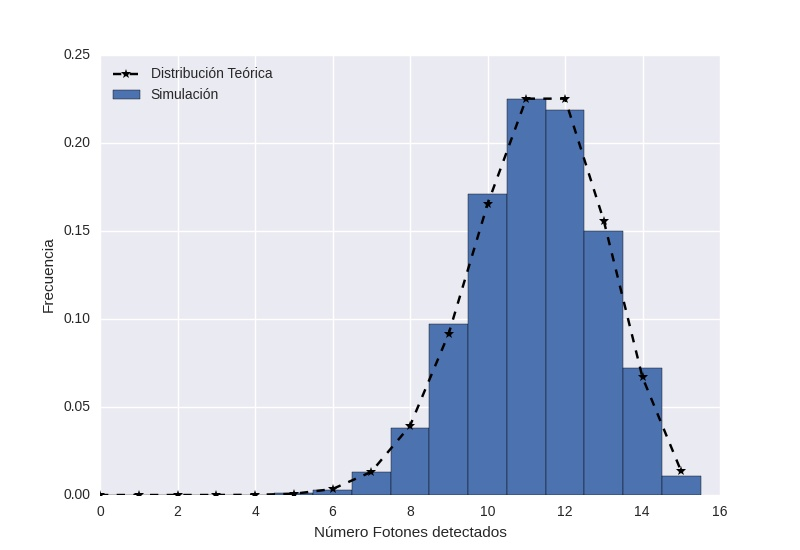
\includegraphics[width=0.75\textwidth]{figb.jpg}
\caption[]{Histograma del item b}
\label{fig:itemb}
\end{figure}

\section{Item c}
Ahora consideremos una funete de intensidad media $I=15\ fot\ s^{-1}$.
La distribución de fotones emitidos en un intervalo de tiempo $t$ seguirá una ditribuión de Poisson.

$$\text{número\ de\ fotones} = \frac{(\lambda t)^k}{k!} e^{-\lambda t}$$

Si consideramos un tiempo $dt=0.001s$ la probabilidad de que uestra fuenta

En un intervalo de tiempo $dt=0.001s$ la probabilidad de emitir  
\begin{figure}
\centering
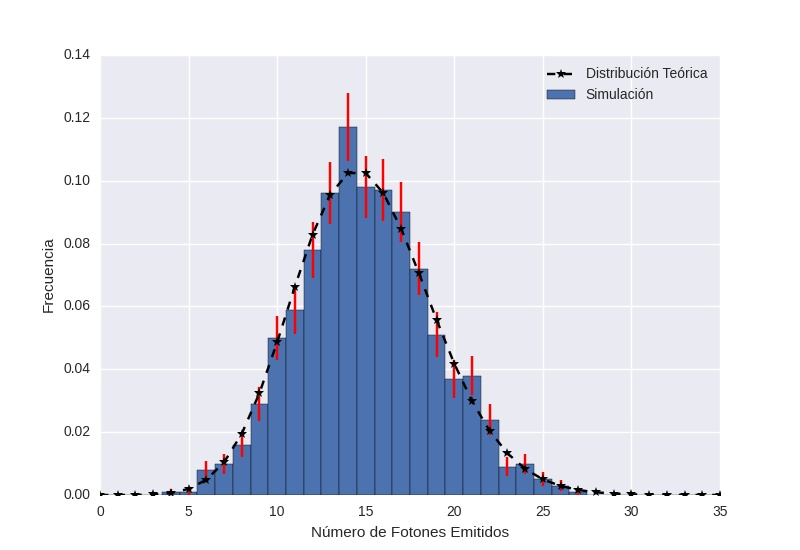
\includegraphics[width=0.75\textwidth]{figc.jpg}
\caption[]{Histograma del item c}
\label{fig:itemc}
\end{figure}

\section{Item d}
\begin{figure}
\centering
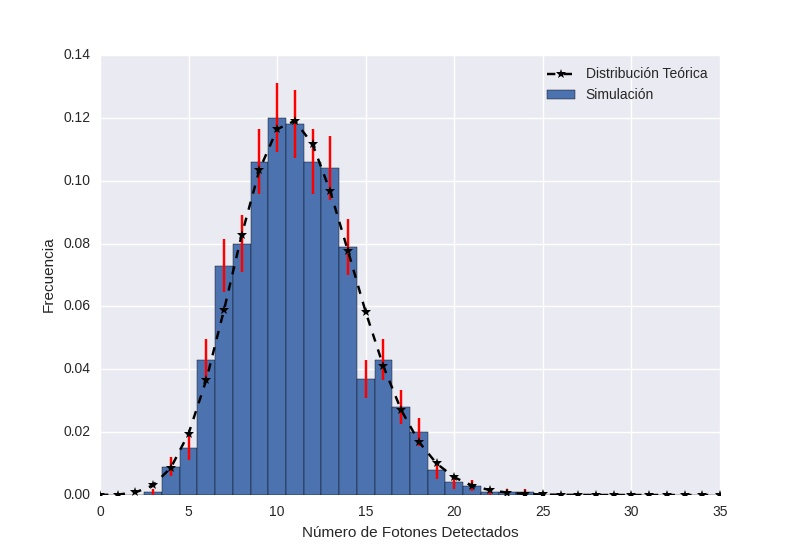
\includegraphics[width=0.75\textwidth]{figd.jpg}
\caption[]{Histograma del item d}
\label{fig:itemd}
\end{figure}

\section{Item e}
\begin{figure}
\centering
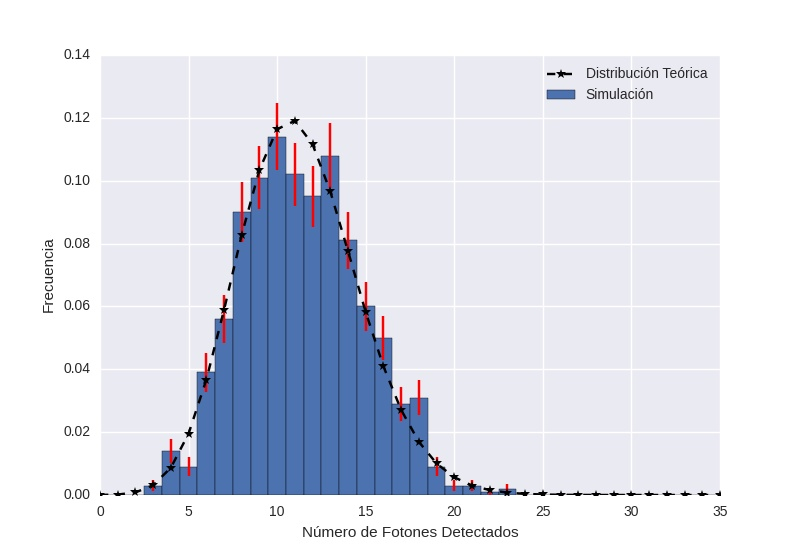
\includegraphics[width=0.75\textwidth]{fige.jpg}
\caption[]{Histograma del item e}
\label{fig:iteme}
\end{figure}

\section{Item f}
\end{document}